%!TEX root=../../../template.tex
\subsection{Ground Station}%
\label{sub:methods_ground_station}

As illustrated by Figure~\ref{fig:general_system_schematic}, the ground
station is the device responsible for:
\begin{enumerate}
    \item Improving positioning precision;
    \item Programming the \gls{UAV}'s trajectory;
    \item Analysing the incoming data.
\end{enumerate}

Now, the first point is handled in automatic fashion by the
\gls{RTK-GPS} devices that are included in the assembly, so there is no
intervention required on my behalf; the second point, flight
programming, is achieved via Arducopter's programming API's. These are
software libraries that allows one to program a drone's flight pattern
using regular programming languages, such as Python. Unfortunately,
there was not enough time for me to learn how this is done. Finally, the
ground station is supposed to process the data that come from the drone.

The \gls{DOAS} software library is a Python package developed
specifically for this thesis data processing operations. It was, as
other components, designed using an \gls{oop} approach and following the
SOLID principles of \acrlong{oop}. This piece of software was written in
response to the initial research that I undertook and that returned no
usable results in terms of modular, compact Python libraries for
\gls{DOAS} applications, that I could use in my work. It is, as far as I
know,  the only \gls{DOAS} solving application with this kind of
structure.

The library (\gls{uml} diagram presented in
Figure~\ref{fig:doas_library}) models a \gls{DOAS} application through
the instrumentation lens. A \gls{DOAS} application is always
parametrised through its spectrometer's physical features and
limitations, which in turn determine the structure of the analysed
spectral data, and even the differential cross sections of the trace
gases that are to be studied. Of course, this library is much more
limited in its capabilities than some specific programs that have become
commonplace in this kind of application, such as
QDOAS~\cite{Danckaert2015}, but the fact that it can be operated through
a Python program and that one can manipulate the data through such tools
as Pandas DataFrames more than make up for this lack. Moreover, since it
is in effect a software library, it is also as flexible as one is
willing to expand it.

\begin{figure}[htpb]
    \centering
    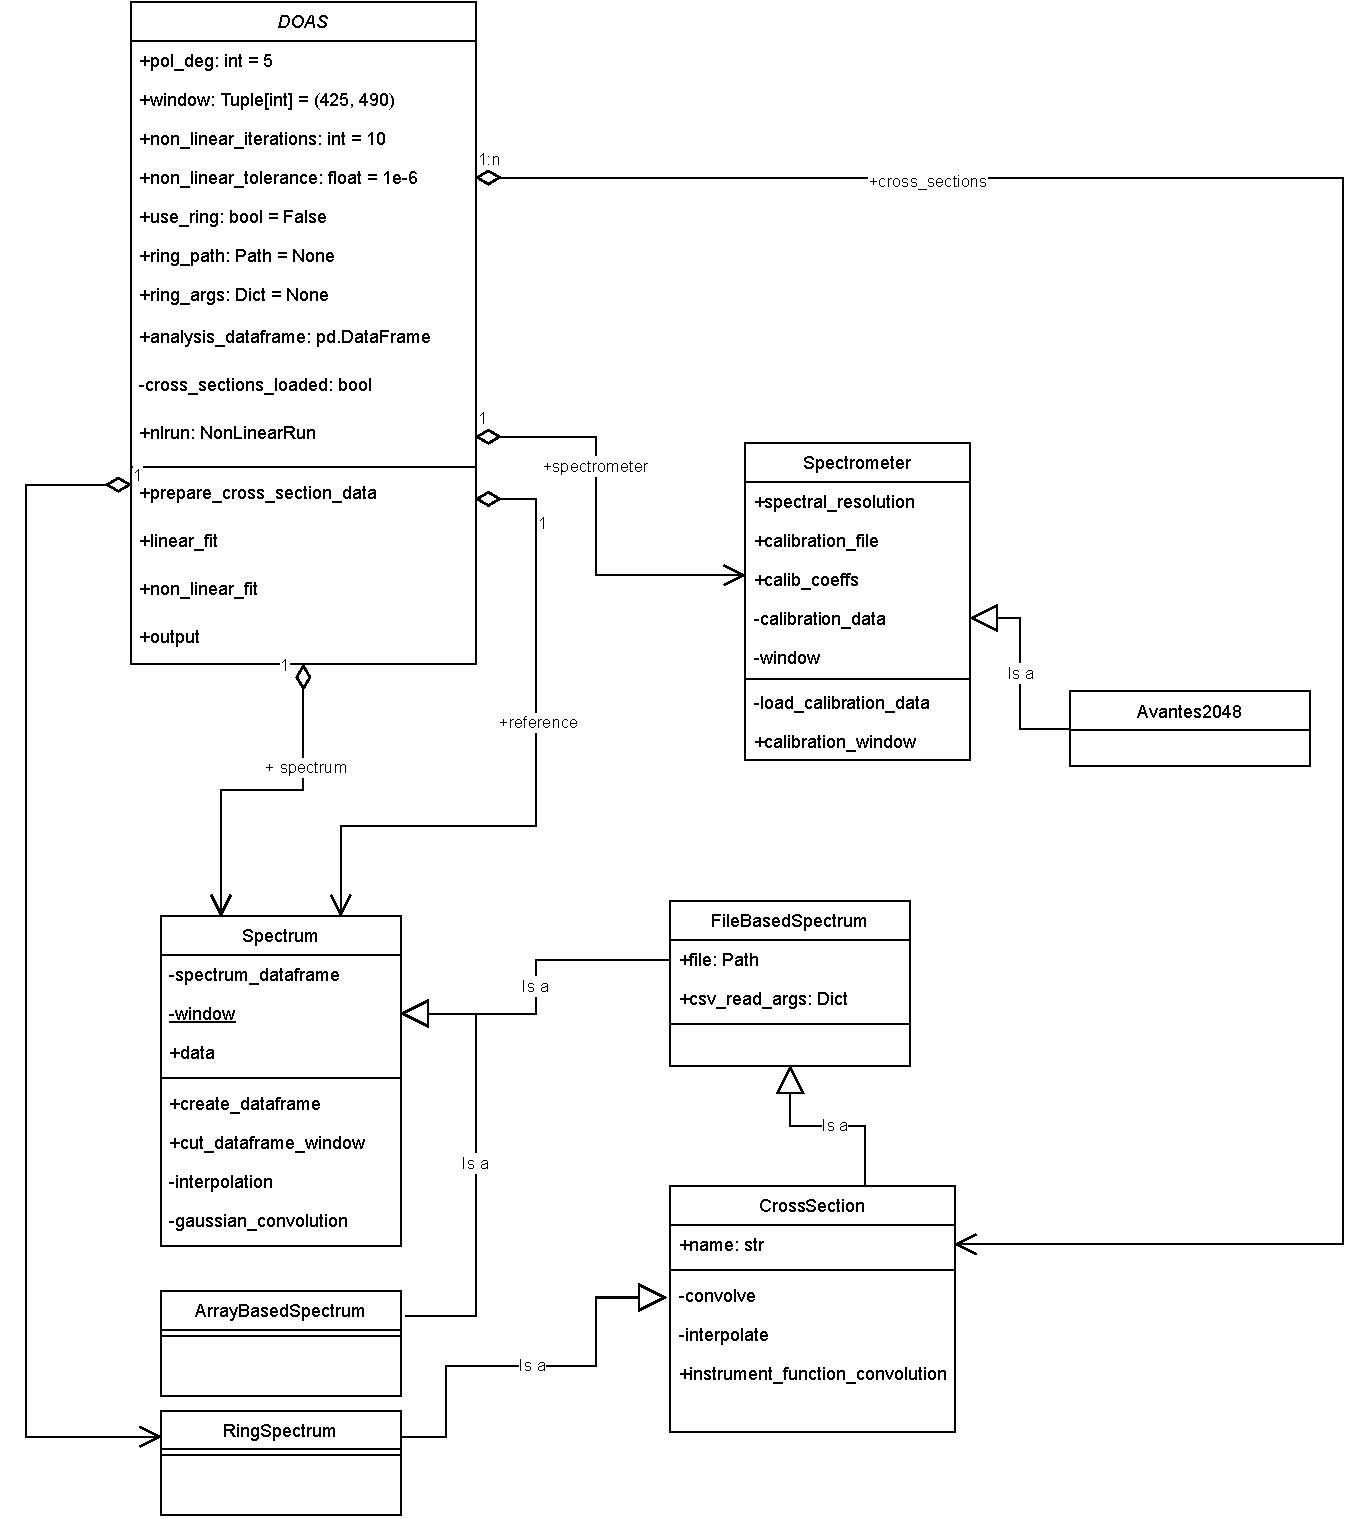
\includegraphics[width=0.8\linewidth]{img/pdf/uml_doas.pdf}
    \caption{UML diagram for the \gls{DOAS} library. The \gls{oop}
    approach that was followed allows for an instrument-oriented
    experiment parametrisation, which is not available in any other
    software}
    \label{fig:doas_library}
\end{figure}

An important side note that attests to this library's relevance is that
it has been fully integrated in FutureCompta's Bee2Fire software, with
further developments being conducted through this team's efforts. This
is the first commercially applicable result provided by the work in this
thesis.


